\documentclass{beamer}
\usetheme{ALUF}

\usepackage[utf8]{inputenc}
% \usepackage{palatino}
% \usepackage[T1]{fontenc}
\usepackage{lmodern}
\usepackage[protrusion=true,expansion=true,tracking=true,kerning=true]{microtype}
\usepackage{graphicx}
\usepackage[utf8]{inputenc}
\usepackage{color}
\usepackage{textcomp}
\usepackage{charter}
\usepackage[T1]{fontenc}
\usepackage[frenchb]{babel}
\usepackage{caption}
\usepackage{pdfpages}
\usepackage{array}
\usepackage{supertabular}
\usepackage{hyperref}
\usepackage{fancyhdr} 
\usepackage{eurosym}
\usepackage{multirow}



\title{24 heures de l'INSA - 44\up{ème} édition}
\subtitle{18 - 20 mai 2017}
\author{Formation Grands Rassemblements}
\date{2 mai 2018}
\institute{Arthur Saunier - 06 25 53 25 79 \\Valentin Godrie - 07 52 62 04 69\\Léo Mouyna - 06 24 30 26 53}

\begin{document}

\begin{frame}[plain,t]
\titlepage
\end{frame}

\begin{frame}% [plain,t]
	\frametitle{Ordre du jour}
\tableofcontents
\end{frame}

%=============================================================================================

%========================================
%PRESENTATION DE LA MANIFESTATION
%========================================

\section{Présentation de la manifestation}

\begin{frame}

\centering\Huge{\textbf{Présentation de la manifestation}}

\end{frame}

\begin{frame}

\frametitle{Généralités}

\begin{tabular}{lcc}
\hline
\multicolumn{3}{|c|}{\centering\Large\textbf{44\up{ème} édition - 18, 19 et 20 mai 2017}}\\
\hline
\\
 & \multirow{4}{*}{\centering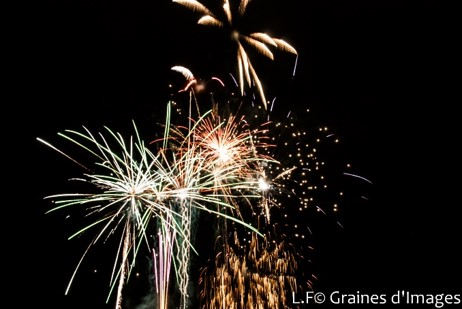
\includegraphics[height=.2\textheight]{Images/Image1}} & \multirow{4}{*}{\centering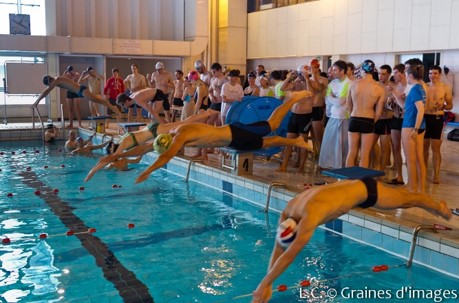
\includegraphics[height=.2\textheight]{Images/Image2}}\\
- 24 heures de courses &\\
- 3 soirs de concerts &\\
\\
- 2 journées d'animations & \multirow{4}{*}{\centering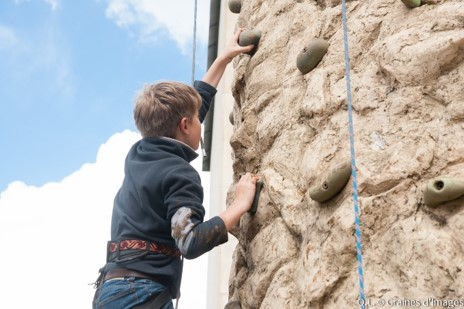
\includegraphics[height=.2\textheight]{Images/Image3}} & \multirow{4}{*}{\centering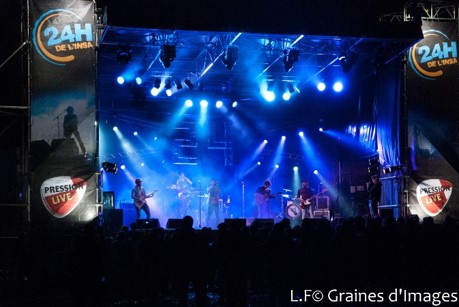
\includegraphics[height=.2\textheight]{Images/Image4}}\\
gratuites&\\
- Environ 30 000 personnes&\\
sur 3 jours &\\
	
\end{tabular}

\end{frame}

\begin{frame}

\frametitle{Les 24 heures en quelques chiffres}

\begin{itemize}
\item \textbf{70} organisateurs toute l'année
\item \textbf{300} organisateurs bénévoles le week-end
\item \textbf{9000} personnes par soirée (2017)
\item \textbf{30 000} personnes attendues sur le week-end
\end{itemize}

\end{frame}

\begin{frame}

\frametitle{Plan général du site}

\centering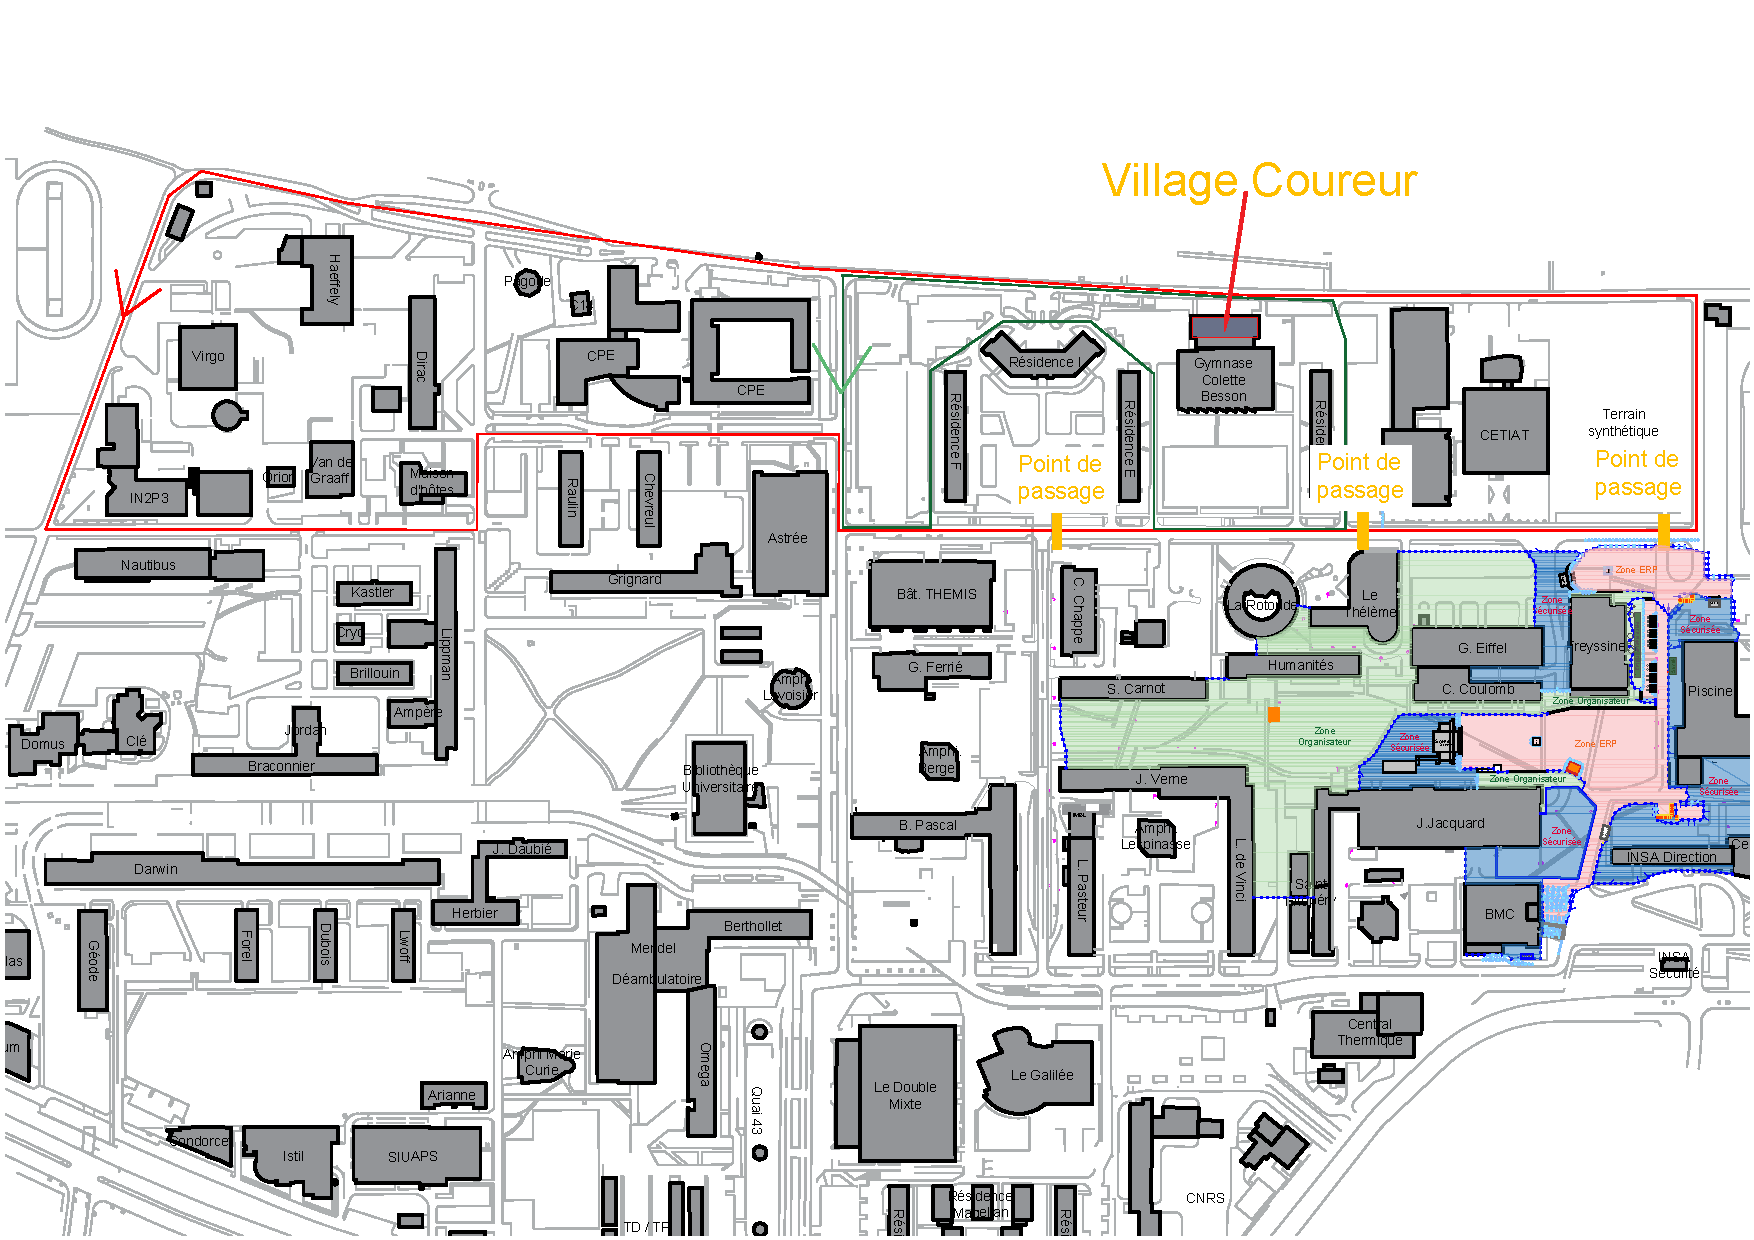
\includegraphics[height=.8\textheight, trim=150 70 0 0,clip]{Exports/Plan_24h_43eme-Parcours_courses}

\end{frame}

\begin{frame}

\frametitle{Organisation}

\centering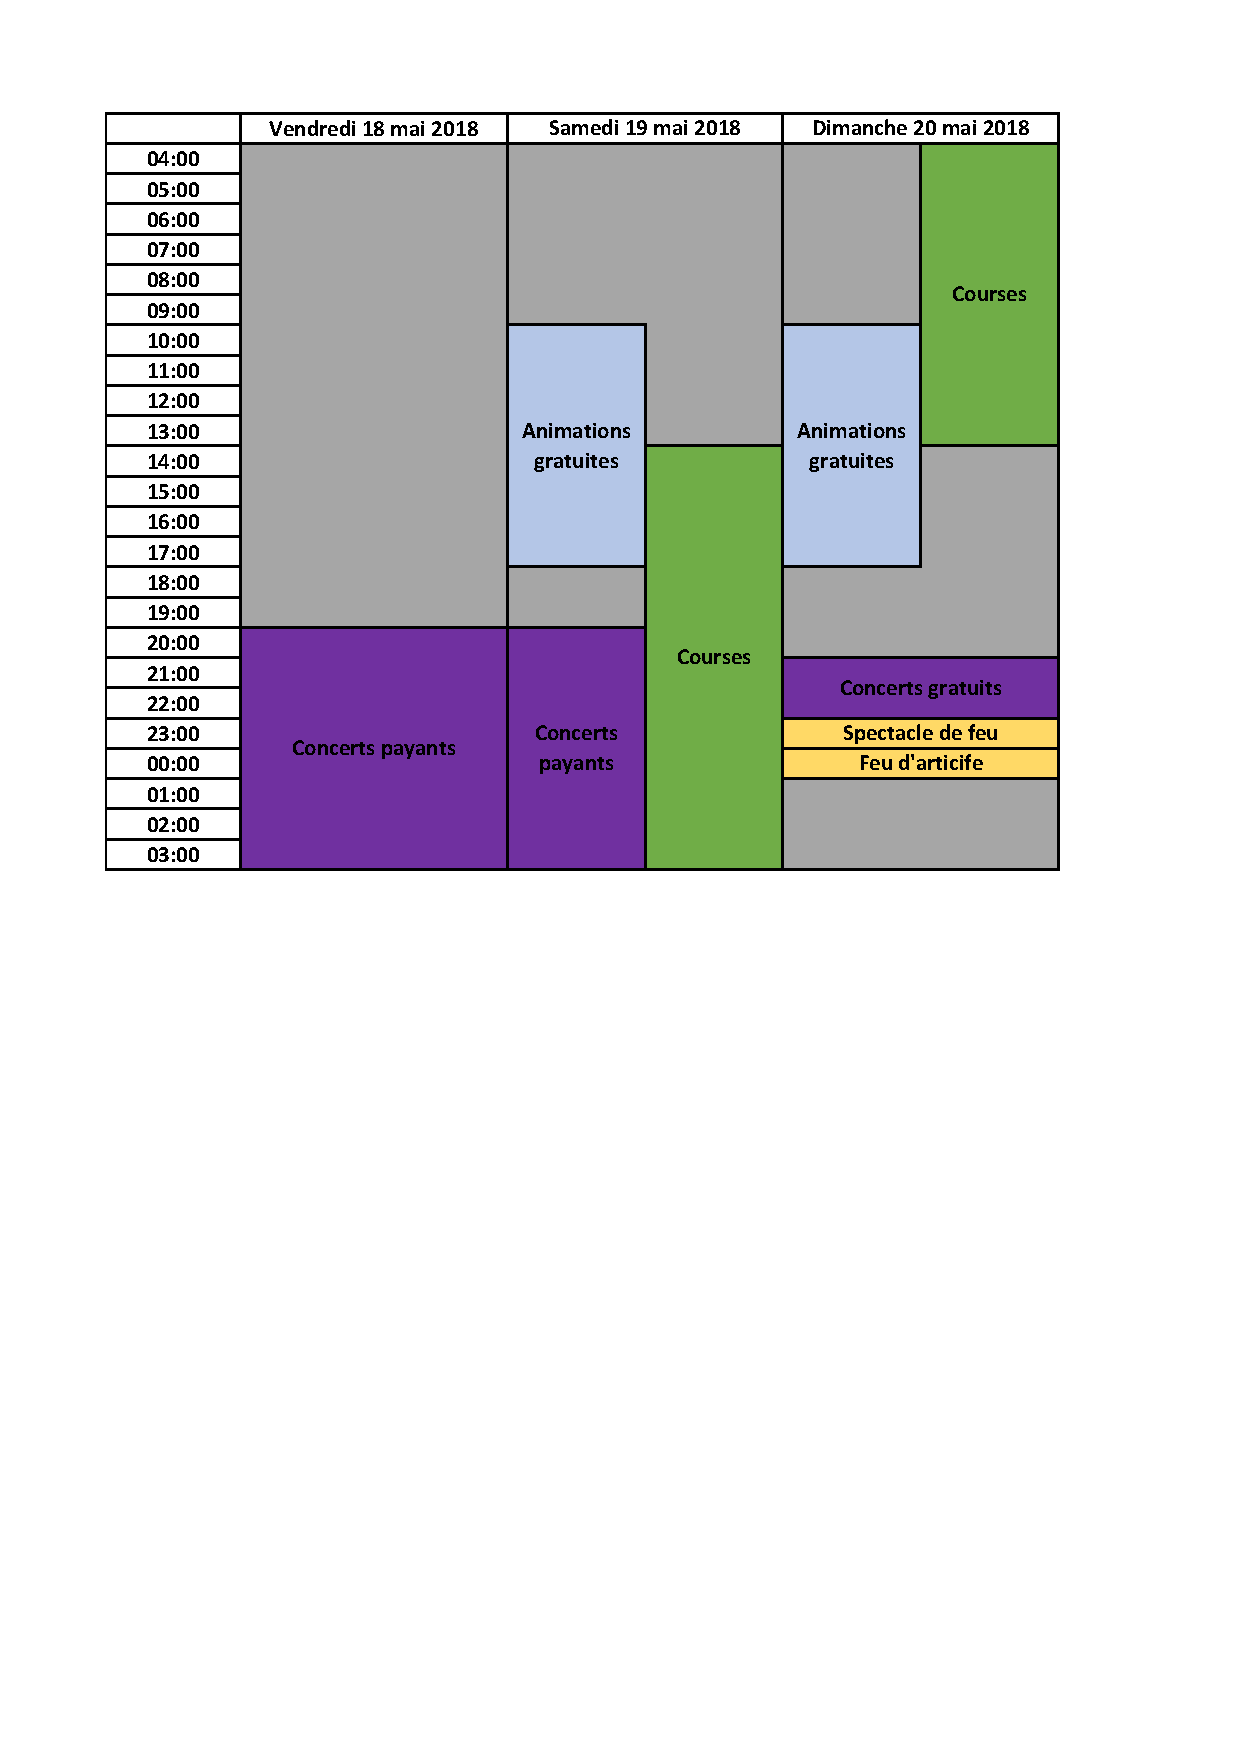
\includegraphics[width=\textwidth]{Images/Timeline}

\end{frame}

%========================================
%BILAN DE L'EDITION 2017
%========================================

\section{Bilan de l'édition 2017}

\begin{frame}

\centering\Huge{\textbf{Bilan de l'édition 2017}}

\end{frame}

\begin{frame}

\frametitle{Nouvelles dispositions}

\end{frame}

\begin{frame}

\frametitle{Remarques générales}

\end{frame}

\begin{frame}

\frametitle{Interventions}

\end{frame}

\begin{frame}

\frametitle{Nouveautés 2018}
\framesubtitle{Prise en compte du bilan 2017}

\end{frame}

%========================================
%DISPOSITIF DE SECURITE
%========================================

\section{Dispositif de sécurité}

\begin{frame}

\centering\Huge{\textbf{Dispositif de sécurité}}

\end{frame}

\begin{frame}

\frametitle{Plans de situation}

\end{frame}

\begin{frame}

\frametitle{Zone ERP}

\end{frame}

\begin{frame}

\frametitle{Dégagements}

\end{frame}

\begin{frame}

\frametitle{Voies pompiers}

\end{frame}

\begin{frame}

\frametitle{Protection contre l'incendie}

\end{frame}

\begin{frame}

\frametitle{Dispositions spécifiques à l'espace restauration}

\end{frame}

\begin{frame}

\frametitle{Troisième scène - Implantation}

\end{frame}

\begin{frame}

\frametitle{Troisième scène - Dispositions de sécurité}

\end{frame}

\begin{frame}

\frametitle{Secouristes - Croix Rouge Française}

\end{frame}

\begin{frame}

\frametitle{Installations électriques}

\end{frame}

\begin{frame}

\frametitle{Zone de caisses}

\end{frame}

\begin{frame}

\frametitle{Grande scène}

\end{frame}

\begin{frame}

\frametitle{Risques météorologiques}

\end{frame}

%========================================
%PROCEDURES D'URGENCE
%========================================

\section{Procédures d'urgence}

\begin{frame}

\centering\Huge{\textbf{Procédures d'urgence}}

\end{frame}

\begin{frame}

\frametitle{Plan d'action en cas d'urgence}

\end{frame}

\begin{frame}

\frametitle{Plan d'accès des secours}

\end{frame}

\begin{frame}

\frametitle{Evacuation des PMR}

\end{frame}

%========================================
%DISPOSITIF DE SURETE
%========================================

\section{Dispositif de sûreté}

\begin{frame}

\centering\Huge{\textbf{Dispositif de sûreté}}

\end{frame}

\begin{frame}

\frametitle{L'équipe sécurité des 24 heures de l'INSA}

\end{frame}

\begin{frame}

\frametitle{Les agents de sûreté (AS)}

\end{frame}

\begin{frame}

\frametitle{Les agents de sûreté (AS) - Zone des caisses}

\end{frame}

\begin{frame}

\frametitle{Dispositions spécifiques liées à la "Travée Verte"}

\end{frame}

\begin{frame}

\frametitle{Prise en compte du plan Vigipirate}

\end{frame}

%========================================
%ACCESSIBILITE
%========================================

\section{Accessibilité}

\begin{frame}

\centering\Huge{\textbf{Accessibilité}}

\end{frame}

\begin{frame}
\end{frame}

%========================================
%PREVENTION SUR LE CAMPUS
%========================================

\section{Prévention sur le campus}

\begin{frame}

\centering\Huge{\textbf{Prévention sur le campus}}

\end{frame}

\begin{frame}
\end{frame}

%========================================
%COURSES ET ANIMATIONS
%========================================

\section{Courses et animations}

\begin{frame}

\centering\Huge{\textbf{Courses et animations}}

\end{frame}

\begin{frame}
\end{frame}

%========================================
%CIRCULATION SUR LE CAMPUS
%========================================

\section{Circulation sur le campus}

\begin{frame}

\centering\Huge{\textbf{Circulation sur le campus}}

\end{frame}

\begin{frame}
\end{frame}



\end{document}
